% find this class at https://archive.danleonard.us/scholarship/coursework/coursework.cls
\documentclass{../../../coursework}

\title{Behavioral Changes to Anthropogenic Environments in Two Species of Macaque}
\subtitle{}
\shorttitle{Macaques in Anthropogenic Environments}
\author{Daniel}{Glenn}{Leonard}
\newdate{date}{18}{12}{2019}
\date{\displaydate{date}}
\course{ANTH}{498}{Senior Capstone Seminar}{University of Illinois at Urbana-Champaign}
\instructor{Dr}{Petra}{E.}{}{Jelinek}
\instructor{Dr}{Brenda}{Margaret}{}{Farnell}

\keywords{urbanization, Anthropocene, urban ecology}
\addbibresource{macaques.bib}
%\addbibresource[location=remote]{https://archive.danleonard.us/scholarship/coursework/illinois/ANTH/498/macaques.bib}
\baseurl{https://archive.danleonard.us/scholarship/coursework/illinois/ANTH/498/macaques.xhtml}

\begin{document}

\maketitle

\begin{abstract}
    Primatology is often conducted in the wild, focusing on elucidating how
    species live in the ecology of their native habitat. As human development
    has increased across the globe, more attention should be paid to how
    primates adapt to the anthropogenic environment. This study reviewed the
    published literature on \textit{Macaca fascicularis} and
    \textit{sylvanus}, comparing quantitative aspects of the species' behavior
    in differing degrees of anthropogenic environments. Anthropogenic
    habitation was expected to lead to greater consumption of human foods,
    smaller home ranges, longer resting times, and larger social groups. In
    \textit{M. fascicularis}, a statistically
    significant relation was found between group size and habitat, but no
    relation was found for the other counts in either species. A call for more
    research into these populations' ecology and behavior is presented.
\end{abstract}

\printkeywords

\section{Introduction}

The sciences of ecology and wildlife biology were born of a sense of
exoticism, a Romanticist question of how the natural world came to be that in
its climax allowed thinkers like Darwin to explore the world in pursuit of
ever more novel findings and ideas \parencite{Nic05}. Today biologists
continue to focus on the pristine, basing their models of species and
ecological change on the ``natural'' world unmolested by human encroachment.
Today, however, humans have changed the face of the planet in many cases
beyond recognition from the ``natural'' order. Despite its frequent dismissal
in ecological study, the human environment has its own ecology and unique
resources that it itself should be considered from an ecological lens. An
analysis of the primatology fieldwork that has heretofore been conducted in
such environments is needed to understand the state of the field.

\subsection{The Anthropogenic World}

Human society has had a profound impact on the ecosystems of the Earth,
radically changing in only a few centuries how wide swaths of the planet,
terrestrial and marine, Accordingly, geologists and climate scientists have
donned the current epoch the ``Anthropocene'' \parencite{Cru00,Lew15}. While
scholars debate the exact onset of this geologic era, whether 8,000 years
before present \parencite{Rud03,Kir05} or as recent as the Industrial
Revolution \parencite{Cru02}, it is indisputable that the majority of
terrestrial life on the planet has been impacted in some way by human
expansion. 

Conservation of the natural environment is a laudable goal, as there is no
better way to protect biodiversity and endangered species than to set aside
undisturbed land \parencite{New95,Hat19}. However, it cannot be denied that
human settlement has drastically reduced the total land area possible for such
undisturbed conservation. The anthropogenic environment is as much a part of
the ecological landscape as is a coral reef, and its study can provide insight
into the evolution and development of populations in an increasingly
human-dominated world.

Despite this pressing need to consider anthropogenic environments, ecology
research -- and primatology in particular -- has persistently remained far
from human environments. Only between 0.4\% and 6\% of ecology research has
been conducted in the 75\% of Earth's ice-free terrestrial surface that
harbors human settlement \parencite{Col00,Mil02}. Conservation biologists' and
ecologists' focus on the idea of a ``wilderness'' leaves the flora and fauna
of cities little understood \parencite{Nie99}, although when population
censuses are taken in cities as developed as Phoenix, Arizona and Baltimore,
Maryland, researchers have been surprised by the diversity present
\parencite{Klo99}.

\subsection{Anthropogenic Environments as Primate Habitats}

Primatologists in particular prefer to conduct research at a small array of
permanent, long-term field sites, which fails to account for the primates who
are not represented \parencite{Bez19}. This model of research has of course
benefits, mainly its desire to maintain relations with the local community and
in its producing comparative and consistent results. Certainly the exotic
field-site model has served conservationists and researchers well in the past
half-century. However, understanding how the subjects of primatology research
fit into the rest of the world is just as -- if not more -- important in the
current global environment.

Most of the prevailing research of the human-nonhuman divide falls into one of
two camps: that of ethnoprimatology or that of interspecies conflict
management. The former primarily looks at the species divide through an
ethnographic lens, in which humans and nonhuman primates together shape a
social space each with shared and distinct roles \parencite{Fue12,Ril13}. The
latter consists of a diverse array of ecological scholarship aimed at reducing
primate endangerment in human environments such as roadways \parencite{Lin16},
analyzing primate effects on cultivated crops \parencite{Hil17,Hoc17,McK15},
and physical conflict \parencite{Hof12}. Recently, researchers have begun to
apply focal-animal sampling techniques to primates in troops that have made
their home ranges either wholly or partially inside heavily developed areas.
Specifically, there is now a wealth of
\textit{Macaca} spp.\ diet and range information
which can be directly compared to research on those same species in less
anthropogenic environments. Urban primate populations that have undergone
recent study include those of \textit{M. sylvanus} in Gibraltar
\parencite{Ethnoprimatology6,Kle17} and Béjaïa \parencite{Mai15} and of
\textit{M. fascicularis} in Singapore \parencite{Kle17}.

\subsection{Hypotheses}

The null hypothesis is the prediction that in all surveyed characteristics,
\textit{M. sylvanus} and \textit{M. fascicularis} individuals do not differ
when in anthropogenic versus wild environments. Four alternative hypotheses
are presented:

\begin{enumerate}

    \item \emph{Anthropogenic-dwelling macaques exhibit a dietary shift with a
    bias toward human foods.} The higher relative availability of human foods
    in such environments provides an ample source of nutrition when the foods
    that make up the animals' natural diets are not obtainable.
    
    \item \emph{Anthropogenic-dwelling macaques exhibit smaller ranges and
    shorter daily path lengths.} Urban and rural human-inhabited areas present
    a higher density of environmental hazards, including vehicular traffic and
    physical conflict with people. It is predicted that in such environments,
    animals would travel less to avoid danger.
    
    \item \emph{Time spent resting is directly correlated with consumption of
    human foods, while time spent feeding is indirectly correlated.} The
    energy density of human foods is often much higher than that of foods
    growing in the wild, as a result of both processing and domestication.
    Macaques that can access such foods regularly may be able to decrease the
    amount of time spent feeding to reach their needed caloric intake.
    
    \item \emph{Anthropogenic-dwelling macaques live in larger social groups.}
    A lack of predation and more reliable access to food are expected to
    reduce a pressure toward small group sizes, allowing macaque groups in
    such environments to grow to larger sizes than would be expected in the
    wild.
    
\end{enumerate}
    
\subsection{Review of Literature}

\subsubsection{Collection of Data}

Due to the frequency with which researchers survey urban populations of the
two species, \textit{M. sylvanus} and \textit{M. fascicularis} were chosen as
the target species for comparison. 13 studies were found to cover at least one
of the two species' behavioral patterns in anthropogenic or ``wild'' habitat.
Data collected from each study, where present, included the environment
(as urban/park, peri-urban, rural, or forest), the percentage of the group's
home range that was anthropogenic, the number (minimum, maximum, and mean) of
individuals, survey method, home range (either MCP or KDE), daily path length,
movement rate, diet (natural: yes, no; refuse: no, minor, extensive;
sanctioned provisioned: no, yes; illicit provisioned: no, minor, extensive;
and raided: no, minor, extensive, also as percentages when available), and
activity budget (percent of time spent resting or feeding).

\section{Results}

\subsection{Data Analysis}

Data were entered into a spreadsheet and analyzed using Microsoft Excel
version 1911. A list of all macaque groups identified is available in
Table~\ref{tab:maindata}.

\subsubsection{Hypothesis 1}
\begin{figure}
    \centering
    \begin{minipage}{0.45\textwidth}
        \centering
        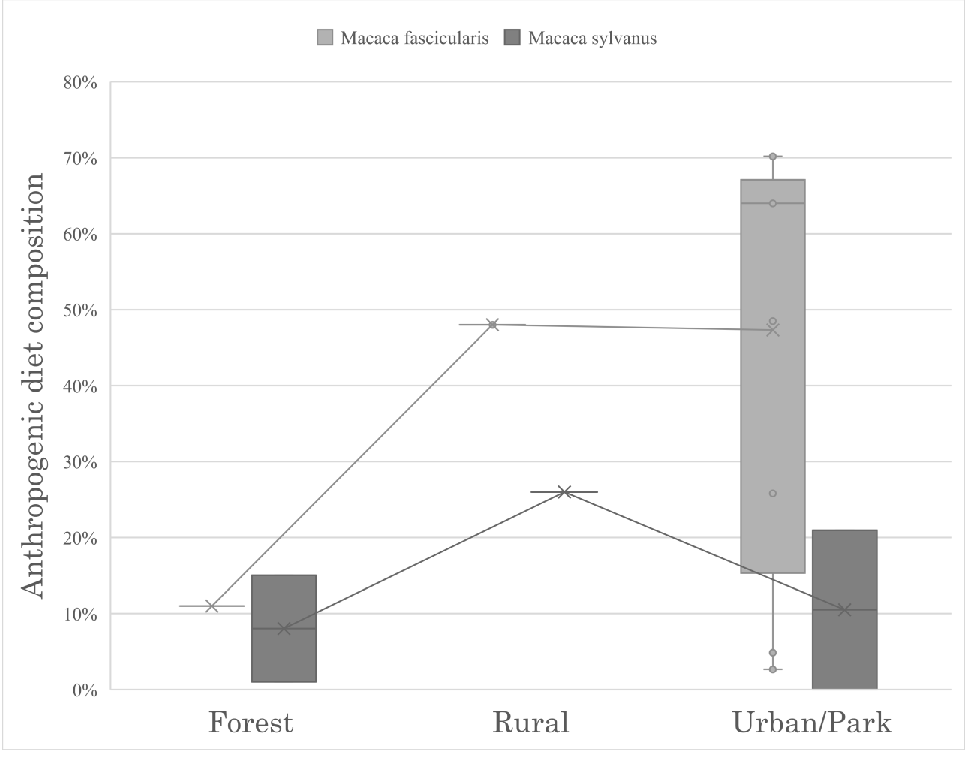
\includegraphics[width=0.9\textwidth]{macaque_table_1.pdf}
        \caption{Dietary Composition of Macaques by Habitat}
        \label{fig:1}
    \end{minipage}\hfill
    \begin{minipage}{0.45\textwidth}
        \centering
        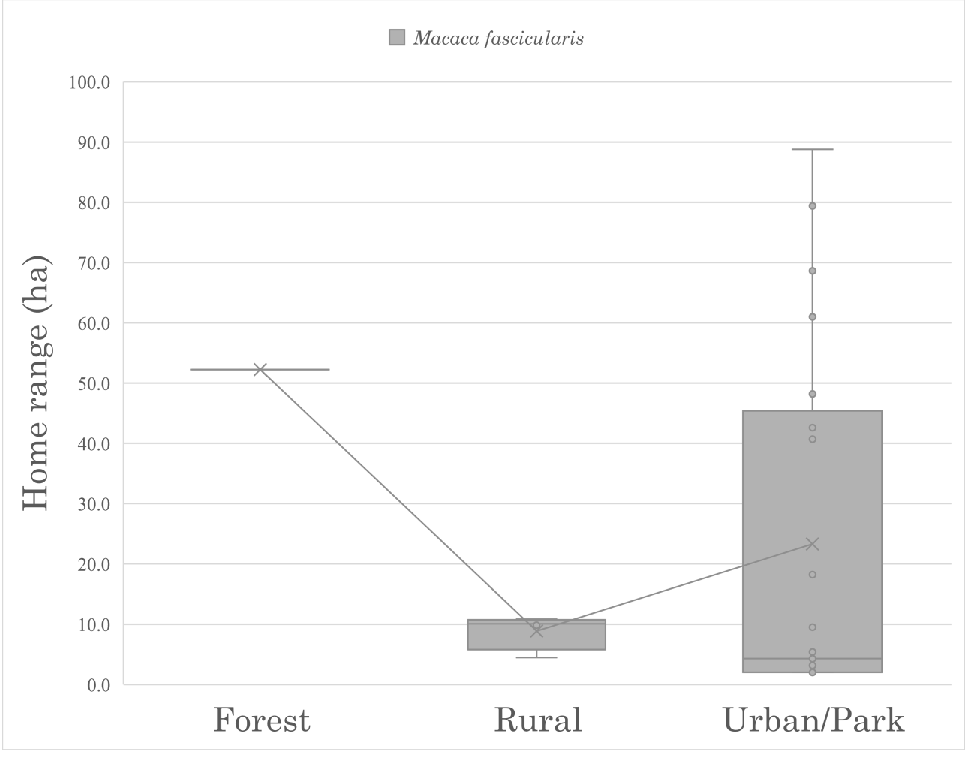
\includegraphics[width=0.9\textwidth]{macaque_table_2.pdf}
        \caption{Home Range Size of Macaque Groups by Habitat}
        \label{fig:2}
    \end{minipage}
\end{figure}

On the question of anthropogenic foods in macaque diets, very little
information was found in studies of forest- or rural-dwelling animals of
either species. Furthermore, there were multiple groups of urban-dwelling
macaques whose anthropogenic food consumption was far lower than expected, and
even lower than some forest groups (\textit{M. fascicularis} min. 3\%,
\textit{M. sylvanus} min. 0\%; see Figure~\ref{fig:1}). The first hypothesis,
that anthropogenic foods are correlated with anthropogenic habitation, is not
accepted.

\subsubsection{Hypothesis 2}

\textit{M. Sylvanus} studies were excluded from home range size comparisons as
they lacked enough data for the three habitat types. In
\textit{M. fascicularis}, while rural home ranges were overwhelmingly smaller
than forest ranges, there was an extremely wide range of urban home ranges
(min. 2.0 ha, mean 4.3 ha, max. 88.8 ha; see Figure~\ref{fig:2}) that overlaps
the ranges for both forest and rural macaques' home ranges. On this count
there is not enough information to accept the second hypothesis.

\subsubsection{Hypothesis 3}
\begin{figure}
    \centering
    \begin{minipage}{0.45\textwidth}
        \centering
        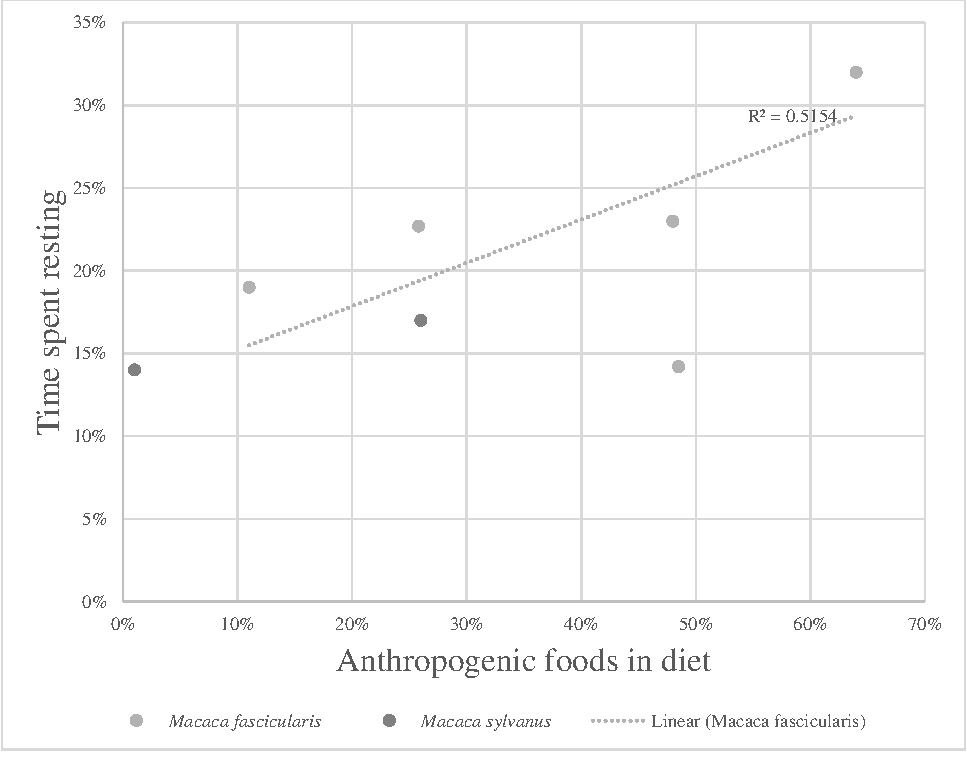
\includegraphics[scale=0.5]{macaque_table_3.pdf}
        \caption{Resting Time as a Function of Anthropogenic Food Consumption}
        \label{fig:3}
    \end{minipage}\hfill
    \begin{minipage}{0.45\textwidth}
        \centering
        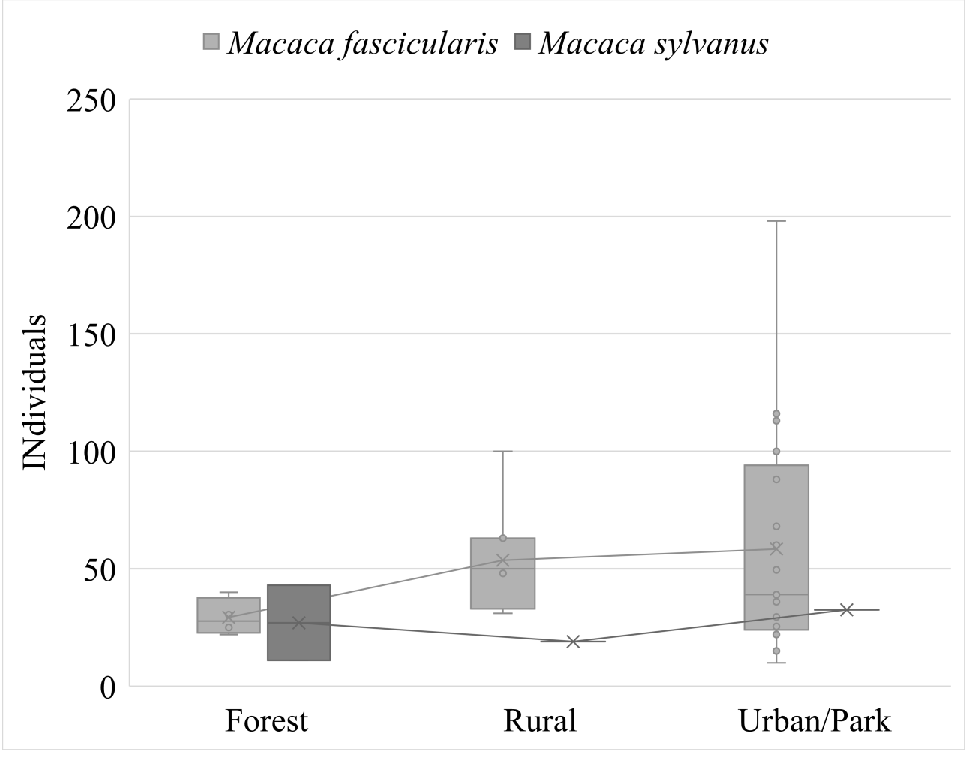
\includegraphics[scale=0.5]{macaque_table_4.pdf}
        \caption{Individuals per Macaque Group by Habitat}
        \label{fig:4}
    \end{minipage}
\end{figure}

Few studies included both the time spent resting and the proportion of
animals' diet deriving from anthropogenic sources, with two and five in
\textit{M. sylvanus} and \textit{fascicularis}, respectively. Making a linear
model is of no use in the two-datapoint set, so only \textit{M. fascicularis}
was analyzed. With a positive trendline and $R^2$ of 0.52, there is tentative
evidence of a correlation between diet and energy expenditure. Without more
data, however, hypothesis 3 cannot be reliably accepted.

\subsubsection{Hypothesis 4}
\begin{figure}
\end{figure}

Of the 53 \textit{Macaca} groups identified from the literature, 19 lacked
censuses of group size. There is not enough data for a conclusive picture of
\textit{M. sylvanus}, but some conclusions may be drawn from the data on
\textit{M. fascicularis}. While forest-inhabiting groups ranged from 22 to 40
individuals in size, urban-dwelling populations existed in a much larger range
of group sizes from 10 to 198 individuals, with most occurring in the 24-94
range. Albeit with large margins of error (see Figure~\ref{fig:4}), there is a
statistically significant (\(p < 0.05\)) result for group size. At least for
\textit{M. fascicularis}, the fourth hypothesis -- that anthropogenic-dwelling
macaques live in larger social groups -- can be tentatively accepted.

\section{Discussion}

It was difficult to find enough primatology studies that had been conducted in
anthropogenic environments, a finding reflective of \citeauthor{Col00}'s
\citeyear{Col00} finding of 0.4\% of ecology research having an urban focus. A
more thorough investigation of which species are most heavily focused on in
such research may allow for a more comprehensive comparison. More importantly,
however, it is necessary to grow the state of the primary literature so that a
more comprehensive understanding of the ecologies of both cities and these
species.

Overall, there is not enough published data to confirm or reject the null
hypothesis, let alone any of the four alternative hypotheses proposed. There
was tentative evidence for hypotheses three and four: a connection between
diet and activity budget and between group size and habitat. On the former, it
is necessary to perform more studies that include both anthropogenic diets and
activity budget, which can allow for a larger sample size in comparisons.
Furthermore, a correlation does not fully explain such a phenomenon. The
energy densities of those specific foods which are eaten by the studied
populations should be evaluated to ensure that the hypothesis is backed with
biological significance. Few studies, even those which described anthropogenic
food consumption, explained which foods the animals were eating, be they
fruits or processed foods. In pursuit of the latter hypothesis, group size
data on \textit{M. sylvanus} would help to allow a cross-species comparison,
but it remains interesting that the group sizes observed have such a wide
range. It is likely that the hypothesis of lower predation allowing larger
group sizes is too simple a model to explain the phenomenon of
anthropogenic-dwelling macaques.

\printbibliography

\newpage
\begin{landscape}
    \centering
    \scriptsize
    \begin{longtabu}{X[L,2]X[1.1]XX[1.25]XXXXXXXX[0.75]X[0.5]XX}
        \noalign{\phantomsection}\caption{Collected literature on \textit{Macaca}~spp.\ behavior.}\label{tab:maindata} \\
        \toprule
        &&&&&&&&& \multicolumn{4}{c}{Food} & \multicolumn{2}{c}{Time spent} \\
        \cmidrule(l){10-13} \cmidrule(l){14-15}
        Source & Species & Location & Name & Habitat & Urban\footnote{Percent of home range occupied by anthropogenic structures} & Individuals & KDE~(ha)\footnote{Home range using KDE} & DPL~(km)\footnote{Daily path length} & Garbage & Provisioned\footnote{Combined managed provisioning and illicit provisions (e.g.\ tourists)} & Raided & Total & Resting & Feeding \\
        \midrule
        \textcite{Mai15} & \textit{sylvanus} & Béjaïa & Les Oliviers & Urban &  & 33 &  &  & No & Moderate & No & 0.21 &  &  \\
            &  &  & Cap Carbon & Forest &  & 43 &  &  & No & Minor & No & 0.15 &  &  \\
        \cmidrule{1-1} \textcite{Kle17} & \textit{fascicularis} & Singapore & SG-BB & Urban & 0.58 &  & 35 & 1.37 & Moderate & Minor &  &  &  &  \\
            &  &  & SG-BNTR 01 & Urban & 0.05 &  & 34.70 & 1.56 & Minor & No &  &  &  &  \\
            &  &  & SG-BNTR 02 & Urban & 0.19 &  & 23.8 & 0.72 & Moderate & Minor &  &  &  &  \\
            &  &  & SG-BTRR & Urban & 0 &  & 42.7 & 0.95 & Minor & No &  &  &  &  \\
            &  &  & SG-MNCF & Urban & 0.11 &  & 40.80 & 2.16 & Moderate & Minor &  &  &  &  \\
            &  &  & SG-RR & Urban & 0 &  & 54.7 & 1.11 & No & Minor &  &  &  &  \\
            &  &  & SG-WW & Urban & 0 &  & 25.9 & 1.53 & Minor & Moderate &  &  &  &  \\
            & \textit{sylvanus} & Gibraltar & GIB-AD & Urban & 0.36 &  & 12.4 & 1.48 & Moderate & Extensive &  &  &  &  \\
            &  &  & GIB-CC & Urban & 0 &  & 9.5 & 1.4 & Minor & Extensive &  &  &  &  \\
            &  &  & GIB-LBI & Urban & 0 &  & 10.8 & 1.09 & Moderate & No &  &  &  &  \\
            &  &  & GIB-MH & Urban & 0.27 &  & 83.3 & 3.46 & Moderate & Moderate &  &  &  &  \\
            &  &  & GIB-PPA & Urban & 0 &  & 13.7 & 1.21 & Minor & Extensive &  &  &  &  \\
            &  &  & GIB-RAW & Urban & 0 &  & 20.10 & 1.6 & Moderate & Extensive &  &  &  &  \\
        \cmidrule{1-1} \textcite{Sha13} & \textit{fascicularis} & Singapore & High & Urban &  & 26 & 9.5 & 1.48 & Moderate & Moderate &  & 0.49 & 0.14 & 0.49 \\
            &  &  & Low & Urban &  & 22 & 18.2 & 1.8 & Minor & Moderate &  & 0.26 & 0.23 & 0.46 \\
        \cmidrule{1-1} \textcite{Ilh17} & \textit{fascicularis} & West Sumatra & A & Urban &  & 36 & 2 &  & Moderate & Moderate &  & 0.7 &  &  \\
            &  &  & B & Urban &  & 28 & 2 &  & Moderate & Moderate &  & 0.7 &  &  \\
            &  &  & C & Urban &  & 68 & 2 &  & Moderate & Moderate &  & 0.7 &  &  \\
            &  &  & X & Urban &  & 15 & 2 &  & Minor & Minor &  & 0.05 &  &  \\
            &  &  & G & Urban &  & 10 & 2 &  & Minor & Minor &  & 0.03 &  &  \\
            &  &  & P & Urban &  & 15 & 2 &  & Minor & Minor &  & 0.03 &  &  \\
        \cmidrule{1-1} \textcite{Won94} & \textit{fascicularis} & Kowloon & E & Urban &  &  & 34 &  &  &  &  &  &  &  \\
        \cmidrule{1-1} \textcite{ElA12} & \textit{sylvanus} & Ozoud Falls & Semi-provisioned & Rural &  & 19 &  &  &  &  &  & 0.26 & 0.17 & 0.28 \\
            &  &  & Wild-feeding & Forest &  & 11 &  &  &  &  &  & 0.01 & 0.14 & 0.26 \\
        \cmidrule{1-1} \textcite{Fue11} & \textit{fascicularis} & Bali & 1 & Rural &  & 31 & 7.2 &  & No & Extensive &  &  &  & 0.23 \\
            &  &  & 2 & Rural &  & 100 & 11 &  & No & Extensive &  &  &  & 0.23 \\
            &  &  & 3 & Rural &  & 63 & 17 &  & No & Extensive &  &  &  & 0.23 \\
        \cmidrule{1-1} \textcite{MdZain2011} & \textit{fascicularis} & Universiti Kebangsaan Malaysia & LF & Urban &  & 60 &  &  & Moderate & Minor &  &  &  &  \\
            &  &  & KBH & Urban &  & 39 &  &  & Moderate & Minor &  &  &  &  \\
            &  &  & KIY & Urban &  & 37 &  &  & Moderate & Minor &  &  &  &  \\
            &  &  & KAB & Urban &  & 23 &  &  & Moderate & Minor &  &  &  &  \\
            &  &  & KRK & Urban &  & 52 &  &  & Moderate & Minor &  &  &  &  \\
            &  &  & KIZ & Urban &  & 30 &  &  & Moderate & Minor &  &  &  &  \\
            &  &  & KKM & Urban &  & 50 &  &  & Moderate & Minor &  &  &  &  \\
            &  &  & PBP & Urban &  & 100 &  &  & Moderate & Minor &  &  &  &  \\
        \cmidrule{1-1} \textcite{Sch121} & \textit{sylvanus} & Gibraltar & AD & Urban &  &  &  &  &  &  &  & 0.77 &  &  \\
            &  &  & PPA & Urban &  &  &  &  &  &  &  & 0.76 &  &  \\
            &  &  & MH & Urban &  &  &  &  &  &  &  & 0.5 &  &  \\
        \cmidrule{1-1} \textcite{Beh14} & \textit{fascicularis} & Bali & TNBBg & Forest & 0.14 & 25 & 32.5 &  & Moderate & No & Minor & 0.11 & 0.19 & 0.34 \\
            &  &  & Nez & Rural & 0.52 & 48 & 6.6 &  & Minor & No & Moderate & 0.48 & 0.23 & 0.27 \\
            &  &  & Tear & Rural & 0.52 & 33 & 5.9 &  & Minor & No & Moderate & 0.48 & 0.23 & 0.27 \\
            &  &  & Temple2 & Rural & 0.52 & 50 & 2 &  & Minor & No & Moderate & 0.48 & 0.23 & 0.27 \\
            &  &  & Scarface & Rural & 0.52 & 50 & 9.5 &  & Minor & No & Moderate & 0.48 & 0.23 & 0.27 \\
            &  &  & Cemetery & Urban & 0.74 & 88 & 1.7 &  & Minor & No & Extensive & 0.64 & 0.32 & 0.21 \\
            &  &  & East & Urban & 0.74 & 113 & 4.10 &  & Minor & No & Extensive & 0.64 & 0.32 & 0.21 \\
            &  &  & Michelin & Urban & 0.74 & 116 & 2.9 &  & Minor & No & Extensive & 0.64 & 0.32 & 0.21 \\
            &  &  & Central & Urban & 0.74 & 102 & 4.40 &  & Minor & No & Extensive & 0.64 & 0.32 & 0.21 \\
            &  &  & Temple & Urban & 0.74 & 198 & 3.4 &  & Minor & No & Extensive & 0.64 & 0.32 & 0.21 \\
        \cmidrule{1-1} \textcite{van99} & \textit{fascicularis} & North Sumatra & A & Forest & 0 & 22 &  &  &  &  &  &  &  &  \\
            &  &  & H & Forest & 0 & 40 &  &  &  &  &  &  &  &  \\
            &  &  & K & Forest & 0 & 31 &  &  &  &  &  &  &  &  \\
        \bottomrule
    \end{longtabu}
\end{landscape}

\end{document}